%!TEX TS-program = lualatex
\documentclass[
	ngerman,
	twoside,
	pdfa=false,
	ruledheaders=section,%Ebene bis zu der die Überschriften mit Linien abgetrennt werden, vgl. DEMO-TUDaPub
	class=report,% Basisdokumentenklasse. Wählt die Korrespondierende KOMA-Script Klasse
	thesis={type=Übung},% Dokumententyp Thesis, für Dissertationen siehe die Demo-Datei DEMO-TUDaPhd
	accentcolor=TUDa-9d,% Auswahl der Akzentfarbe
	custommargins=false,% Ränder werden mithilfe von typearea automatisch berechnet
	marginpar=false,% Kopfzeile und Fußzeile erstrecken sich nicht über die Randnotizspalte
	%BCOR=5mm,%Bindekorrektur, falls notwendig
	parskip=half-,%Absatzkennzeichnung durch Abstand vgl. KOMA-Sript
	fontsize=11pt,%Basisschriftgröße laut Corporate Design ist mit 9pt häufig zu klein
%	logofile=tuda_logo.pdf, %Falls die Logo Dateien nicht installiert sind
]{tudapub}

% Sprachanpassung
\usepackage[english, main=ngerman]{babel}
\usepackage[autostyle]{csquotes}
\usepackage{microtype}
\usepackage{listings}
\usepackage{array}

% Literaturverzeichnis
\usepackage{biblatex}
\addbibresource{literature.bib}

% Pakete-Mathematik & mehr
\usepackage{mathtools}
\usepackage{amsmath}
\usepackage{amsfonts}
\usepackage{subcaption}
\usepackage{color}

% neu cmds
\newcommand*\diff{\mathop{}\!\mathrm{d}}
\newcommand*\Diff[1]{\mathop{}\!\mathrm{d^#1}}


\begin{document}
	\title{Software Engineering Übung 09}
	\subtitle{Maintenance}
	\author[J. Lippert \and M. Dierking]
	{Jonathan Lippert \and Magnus Dierking}
	%\reviewer{}
	%\department{ce}

	
	\submissiondate{\today}
	

	\maketitle
	\pagenumbering{gobble}


	% Kurzzusammenfassung
%	\include{chapters/zusammenfassung}

	% Inhaltsverzeichnis 
%	\tableofcontents
	\newpage
	\pagenumbering{arabic}
	\setcounter{page}{1}
	

%-------------------------------------------------------------------------------------------------
     \chapter{Feature Diagram}


\begin{figure}[h!]
	\centering
	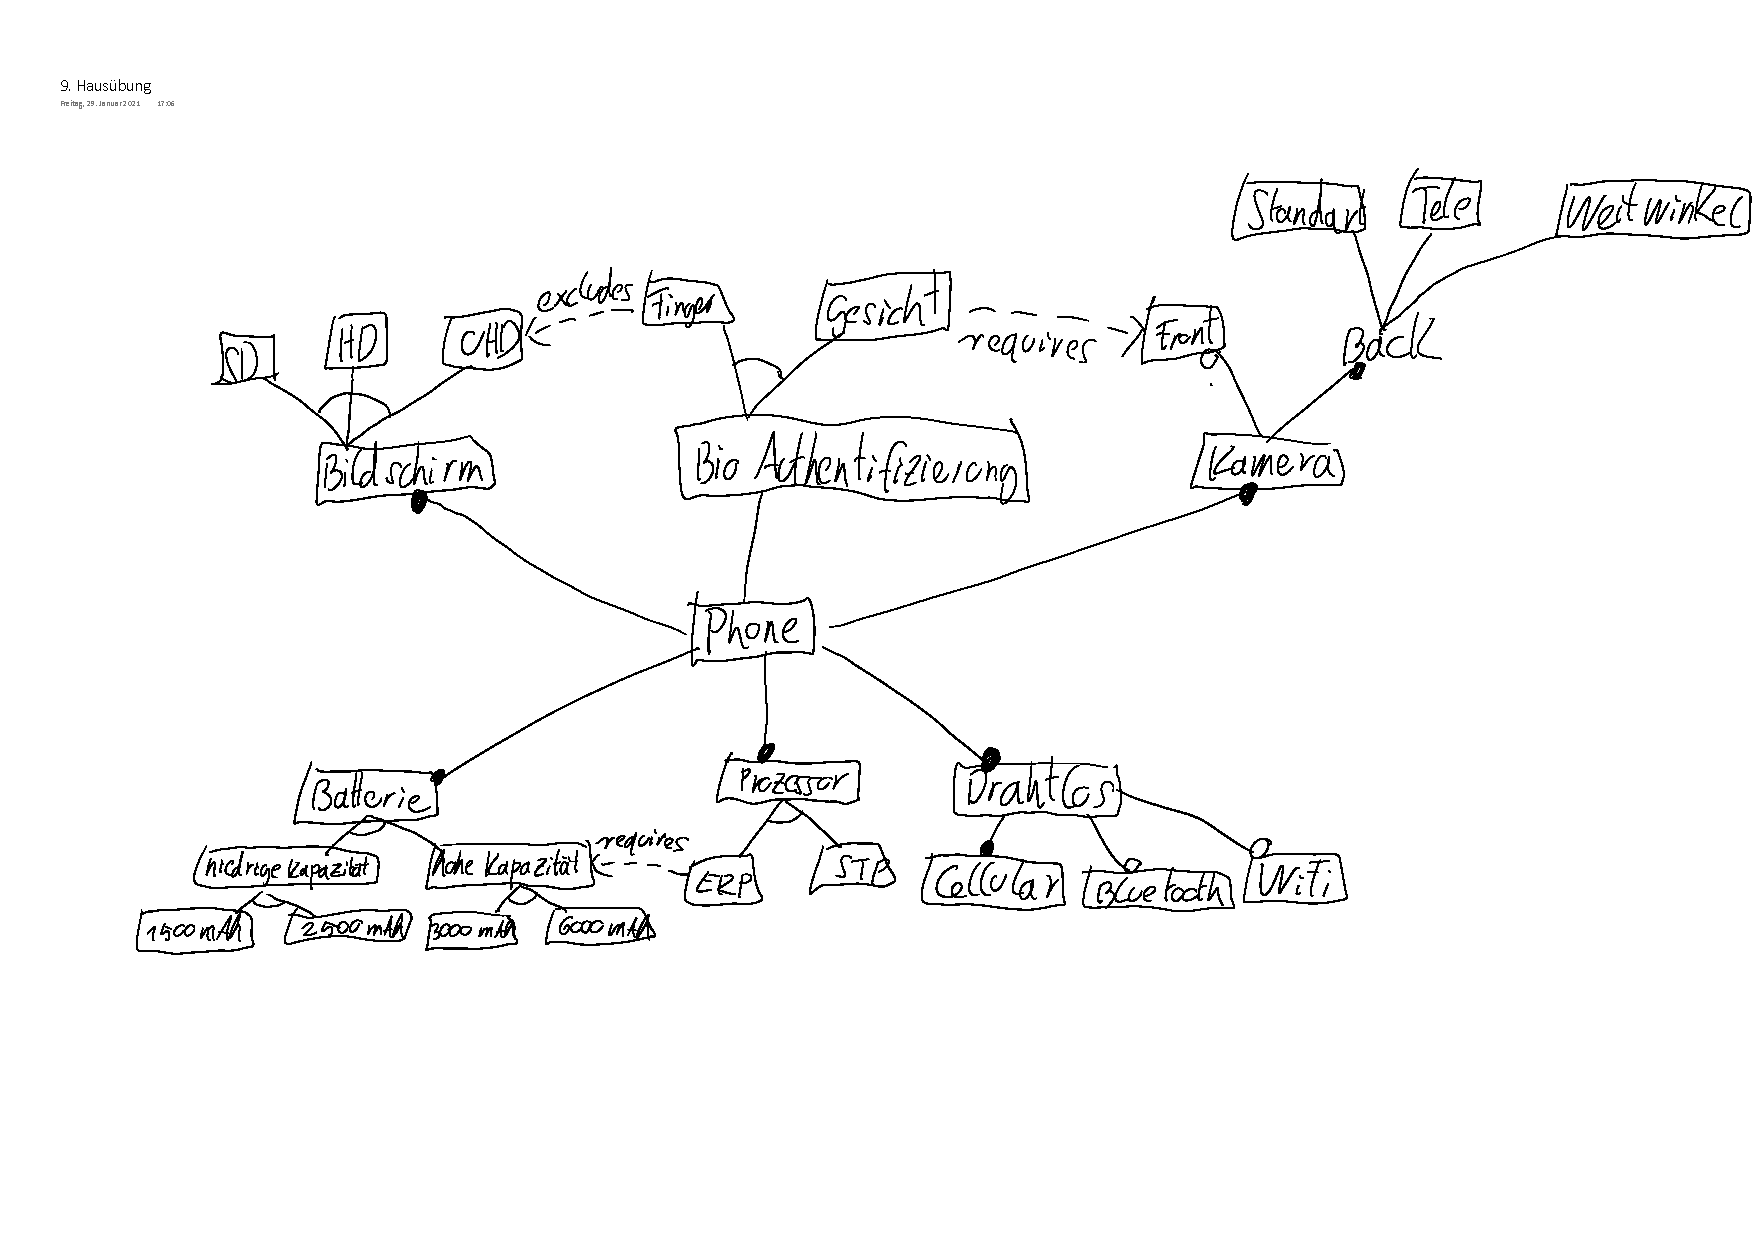
\includegraphics[width=0.8\textwidth, clip]{images/9Hausuebung_SW.pdf}
	\caption{Feature Diagramm des CYOD-Phones.}
	\label{fig:graphLCOM}
\end{figure}

     \chapter{Feature Diagramm Constraints}

	
%-------------------------------------------------------------------------------------------------

	% Literaturverzeichnis
	\printbibliography % Erstellt die Bibliography
	
%	\include{chapters/anhang}
	

\end{document}